%MARCOS RIAL DOCAMPO
%Parte del documento principal TFG

%%%%%%%%%%%%%%%%%%%%%%%%%%%%%%
%% CAPÍTULO 1. INTRODUCCIÓN %%
%%%%%%%%%%%%%%%%%%%%%%%%%%%%%%


\chapter{Introducción}
\label{cap:introduccion}

\section{Marco Global}
Antes de comenzar conviene diferenciar los términos mangle y manglar. Comúnmente se conoce como mangle a la especie forestal (árbol o arbusto) que crece en el ecosistema del manglar o también llamados bosques de mangle (figura \ref{fig:mangle}). Por lo tanto, en este documento se hablará de especies de mangle y se recurrirá al manglar o bosque de mangle para determinar la zona en la que viven estas especies.\Sep

\begin{figure}
	\centering
	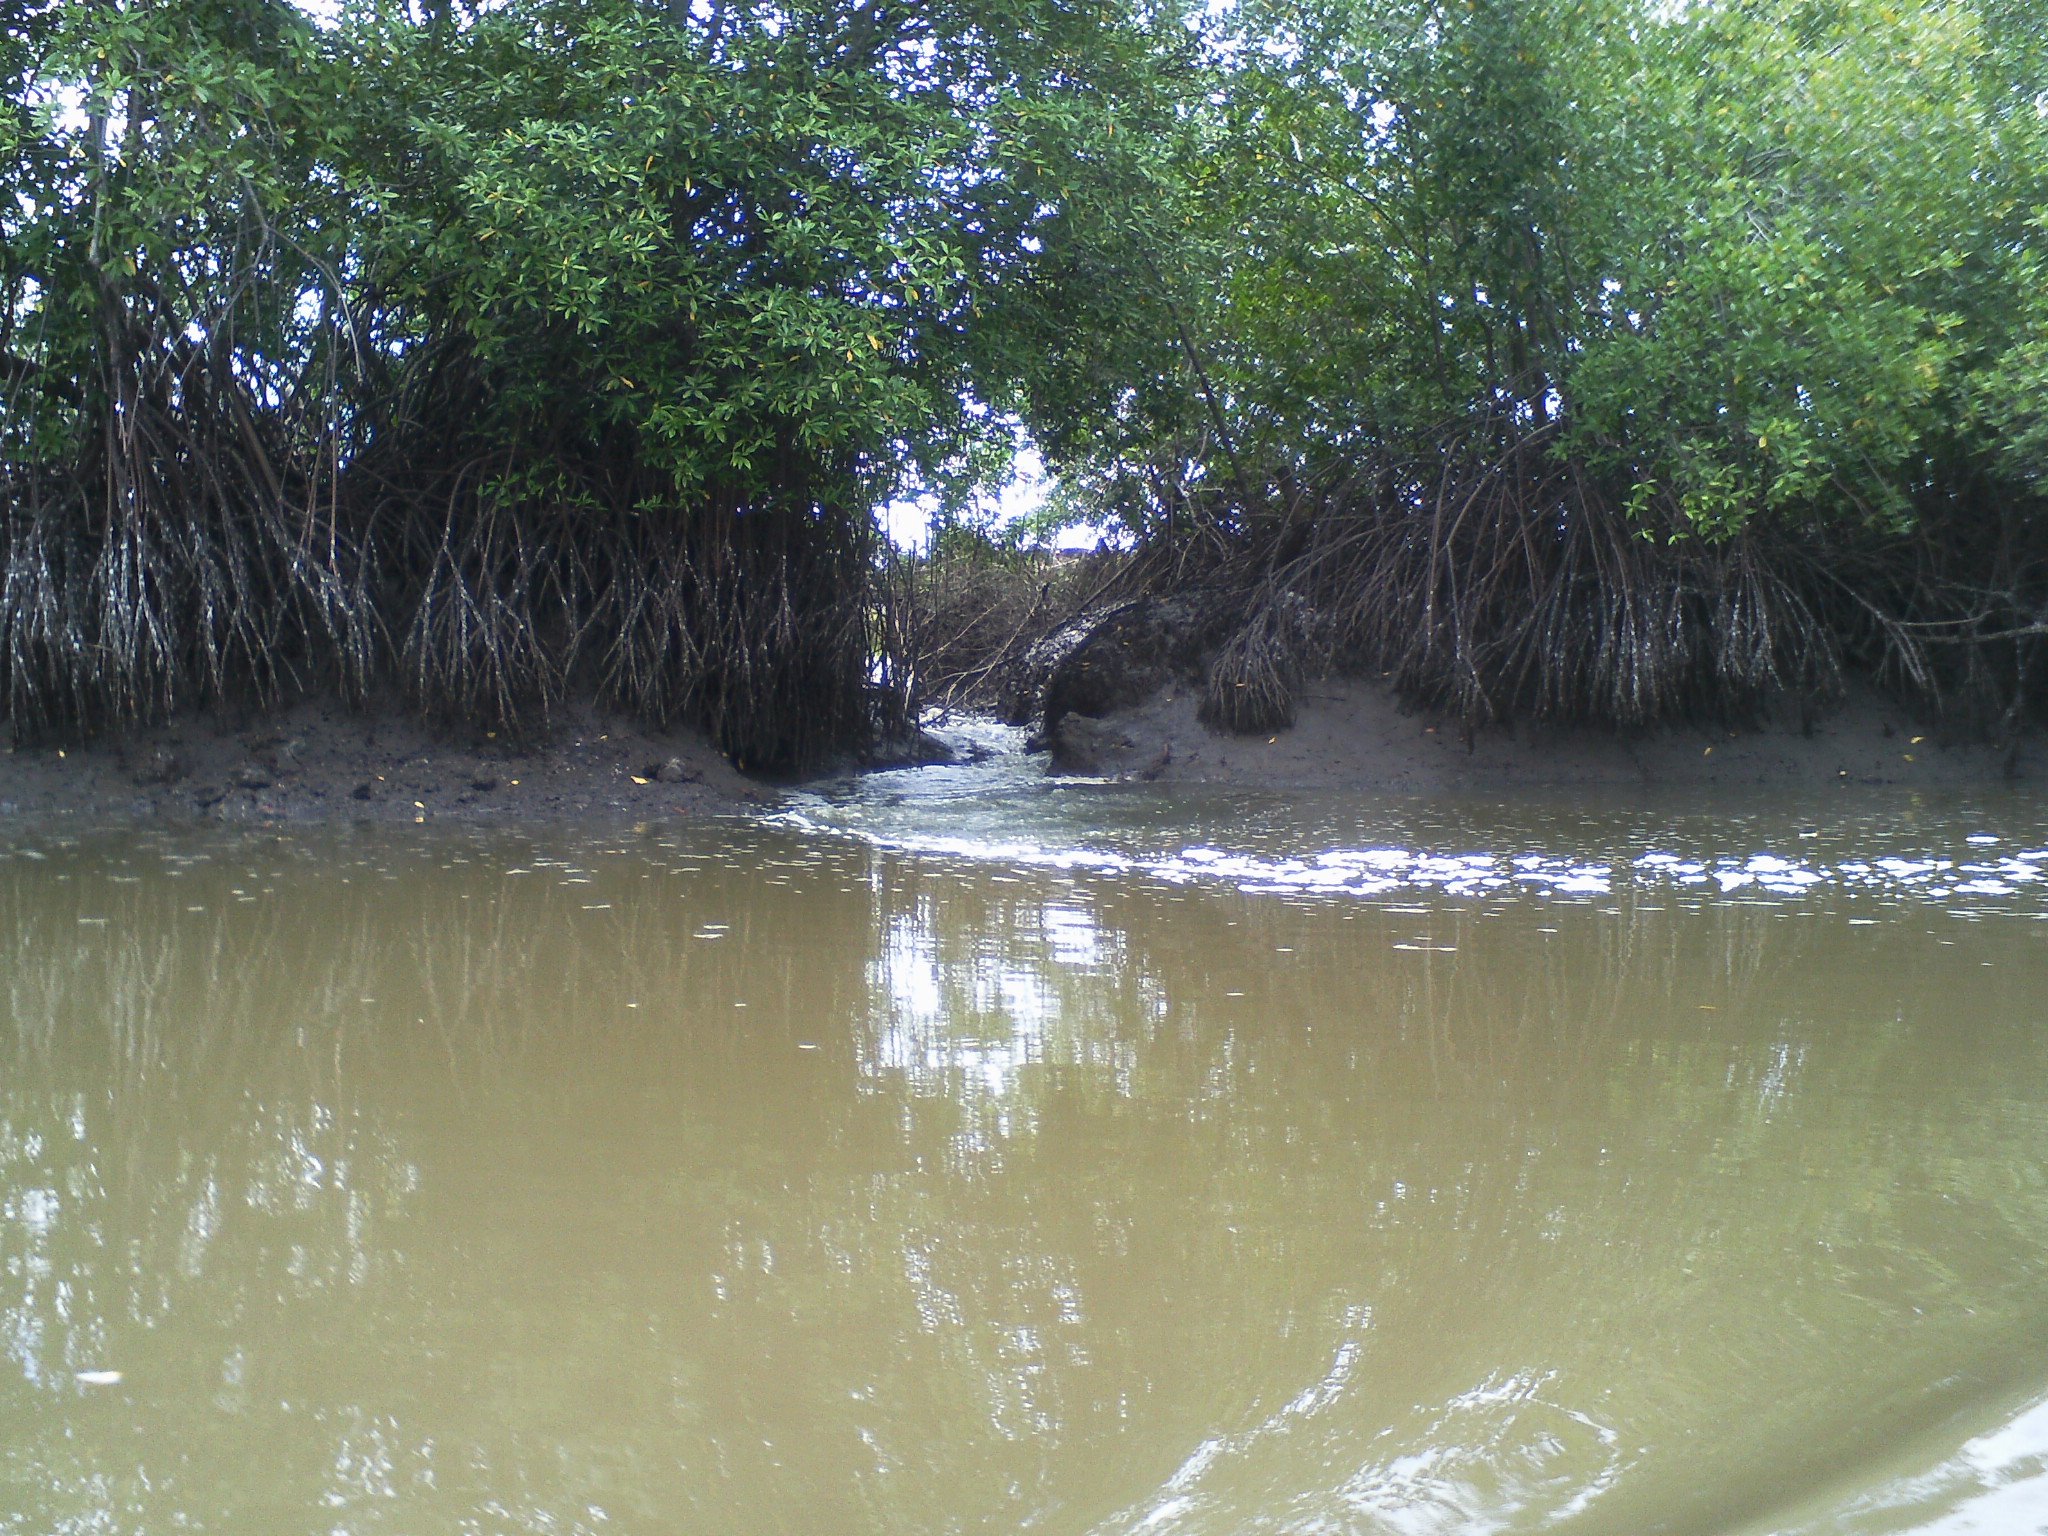
\includegraphics[width=0.7\linewidth]{./Imagenes/Mangle2.eps}
	\captionsetup{font={footnotesize,it}}
	\caption[Mangle en el Golfo de Fonseca]{Aspecto del mangle en un estero del Golfo de Fonseca. Fotografía de Rafael Enrique Corrales.}
	\label{fig:mangle}
\end{figure}

Los manglares componen en la costa de centroamérica uno de los sistemas medioambientales más extensos y complejos del mundo. Situados en la zona intermareal próxima a las desembocaduras de los ríos o esteros, están compuestos por más de 80 especies diferentes de árboles y siendo hábitat de más de 2000 especies de animales, algunas de ellas migratorias.\Sep

La importancia ecológica y comercial de este sistema propio de zonas tropicales y subtropicales, como se muestra en la figura \ref{fig:mundial}, es notable puesto que previenen la erosión de la línea de costa y sirven como sustento económico de la población en forma de producción de la industria pesquera y aporte de madera, leño y carbón \citep{Lara1999}.\Sep

Centroamérica posee muchos kilómetros de costa en relación a su área territorial, con relaciones cercanas a que por cada kilómetro de costa existen $80km^{2}$ de continente y cerca del 70\% de su población vive a menos de 100 km de la costa. Estos datos representan, más si cabe, la importancia de estas zonas para la población y da una idea de su valor económico.\Sep

\begin{figure}
	\centering
	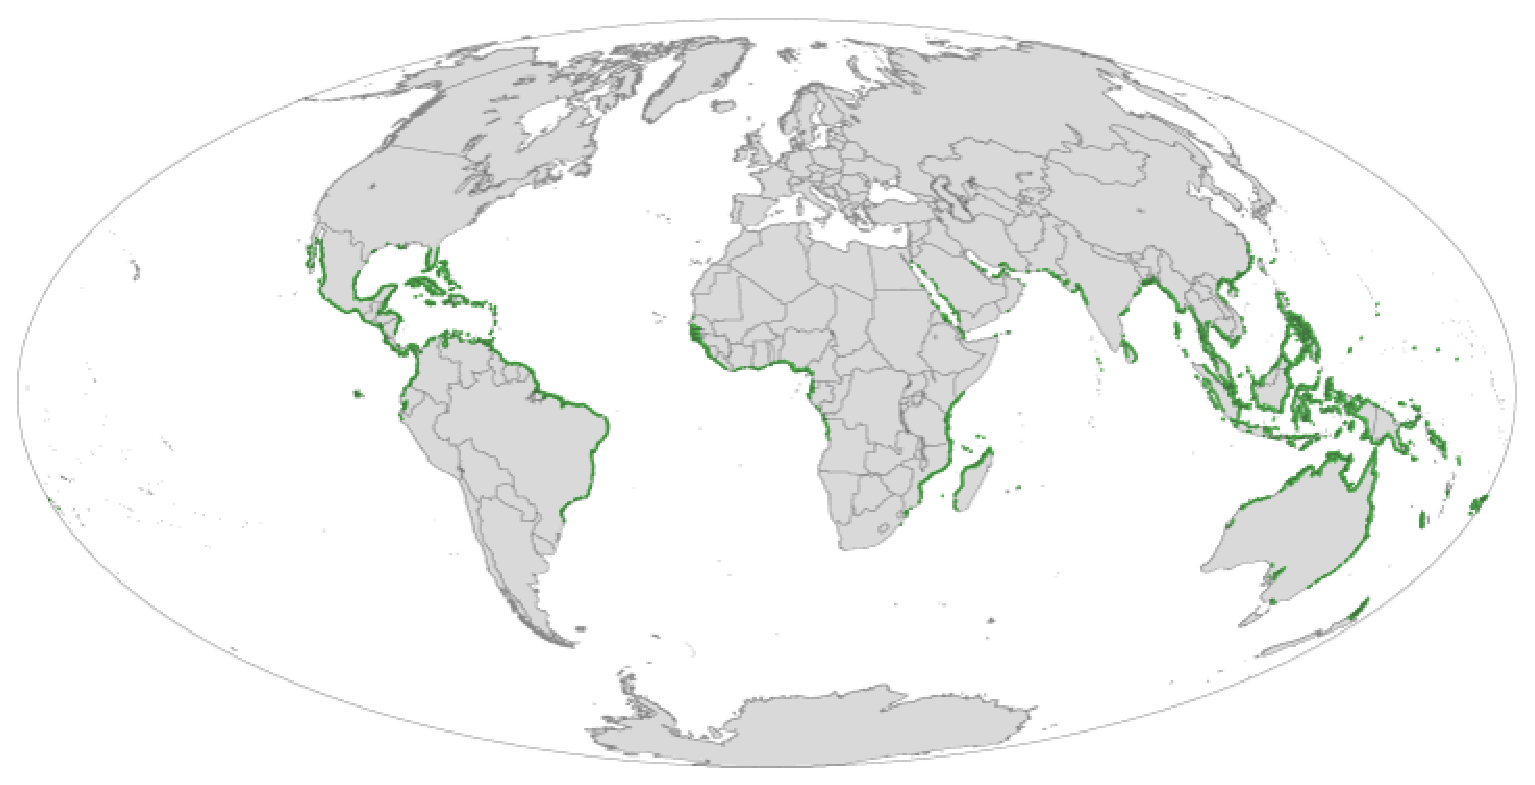
\includegraphics[width=0.8\linewidth]{./Imagenes/distribucion_mundial_mangle.eps}
	\captionsetup{font={footnotesize,it}}
	\caption[Distribución mundial de manglar]{Distribución mundial del manglar. Fuente: Wikimedia Commons.}
	\label{fig:mundial}
\end{figure}

El manglar es un ecosistema delicado y dependiente de los procesos que ocurren fuera de sus fronteras, como pueden ser cambios en las escorrentías de los ríos que afectan a estas zonas, alteraciones en la calidad del agua, provocadas por ejemplo por contaminantes arrastrados por la deriva, o porcentaje de salinidad de las aguas. Esto convierte a mareas, ríos y corrientes litorales como principales agentes alteradores del ecosistema manglar, pero también existe una componente humana importante que afecta directamente.\Sep

Los bosques de mangle de esta región están compuestos por bosque de mangle alto y bosque de mangle bajo. El bosque alto es el situado sobre la línea de costa y su altura varía entre los 5 y los 10 metros, mientras que el bosque bajo se sitúa contiguo al alto en zonas más cercanas a tierra. En el bosque de mangle alto conviven las especies \textit{Rhizophora mangle} y \textit{Laguncularia racemosa}. En el bosque de mangle bajo conviven mayormente las especies \textit{Avicennia germinans} y \textit{Conocarpus erectus}. Estas especies, excepto la última, serán descritas más adelante en el capítulo de Materiales y Métodos (\ref{cap:materialymetodos}).\Sep

En cambio, el manglar es un ecosistema gravemente amenazado. Como se mencionaba, el impacto ambiental, directo e indirecto, no solo procede de la creación de infraestructuras, expansión urbana y desarrollo de industria petrolera sino también de la reconversión en zonas de cría de camarón (figura \ref{fig:camaroneras}) o agricultura costera y salinas (figura \ref{fig:salinas}) que deterioran la calidad del agua. Otras causas del deterioro a escala global de los manglares serían la escasa legislación de la propiedad de recursos naturales, los cambios de actividad de las comunidades costeras, las malas decisiones políticas, la ausencia de planes de desarrollo costero, la depreciación del valor ecológico, la explotación no sostenible o el desconocimiento de las consecuencias \citep{yanez1994}.\Sep

\begin{figure}
	\centering
	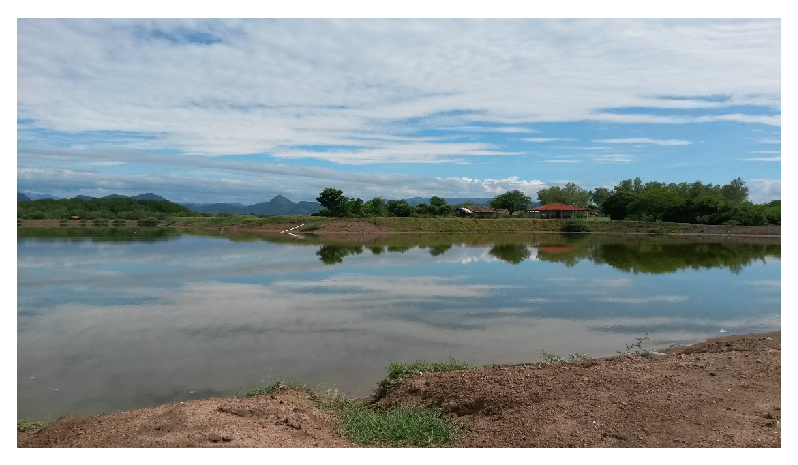
\includegraphics[width=0.9\linewidth]{./Imagenes/Camaronera2.eps}
	\captionsetup{font={footnotesize,it}}
	\caption[Estanques de cría de camarón]{Estanques dedicados a la cría de camarón en el Golfo de Fonseca. Fotografía de Rafael Corrales Andino.}
	\label{fig:camaroneras}
\end{figure}

Una de las posibles soluciones que mitiguen estas causas es la de conocer mejor este ecosistema y su funcionamiento. Precisamente esta es una de las finalidades de este \ac{TFG}.\Sep

El empleo de sensores remotos para proyectos relacionados con el medioambiete y el entorno forestal es una realidad y se han utilizado mucho estas últimas décadas con unos buenos resultados. Como por ejemplo, \cite{bodart2011pre} y \cite{cajacuri2011medicion} realizan un estudio multitemporal de los cambios sufridos por las coverturas forestales, mientras que el estudio de \cite{chen2013multi} se centra precisamente en analizar los cambios en el bosque de mangle hondureño apoyándose en imágenes Landsat. \cite{lee2009applying} destacan la utilización de sensores remotos por la velocidad y precisión a la hora de recabar datos y comparan la utilización de diferentes sensores.\Sep

\begin{figure}
	\centering
	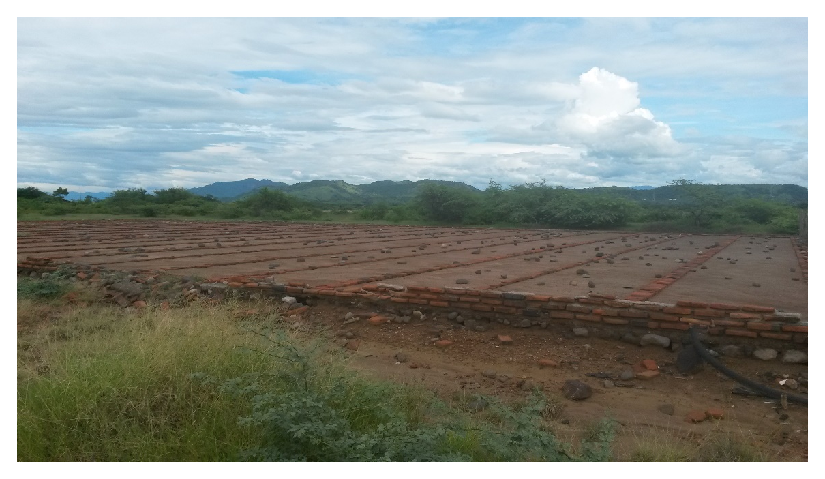
\includegraphics[width=0.9\linewidth]{./Imagenes/Salineras.eps}
	\captionsetup{font={footnotesize,it}}
	\caption[Salineras]{Extensión de terreno dedicada a la producción de sal. Fotografía Rafael Enrique Corrales.}
	\label{fig:salinas}
\end{figure}

\section{Objetivos}
\subsection{Objetivo general}
El objetivo general del trabajo es el de evaluar la posibilidad de emplear imágenes obtenidas con sensores remotos para diferenciar las distintas especies de mangle que se encuentran en el Golfo de Fonseca.\Sep

De todas las especies de mangle existentes en el Golfo de Fonseca se ha decidido tomar tres para este estudio por ser las más predominantes. Son las siguientes:

\begin{itemize}
	\item Mangle Rojo. Nombre científico \textit{Rhizophora mangle} \citep{JimenezRhizophora}.
	\item Mangle Blanco. Nombre científico \textit{Laguncularia racemosa} \citep{JimenezLaguncularia}.
	\item Mangle Prieto. Nombre científico \textit{Avicennia germinans} \citep{JimenezAvicennia}.
\end{itemize}

La hipótesis desde la que se parte es que la respuesta espectral de las diferentes especies de mangle sea lo suficientemente diferente para que este objetivo se cumpla. Esto conduce a la realización de unos objetivos específicos en los que se busca concretar más en el trabajo.

\subsection{Objetivos específicos}
Los objetivos específicos serán el análisis de separabilidad espectral de las especies de mangle del Golfo de Fonseca y determinar la utilidad potencial del empleo de imágenes Landsat para diferenciar las especies analizadas.\Sep

Una vez realizado el análisis de especies se aplicarán los datos extraídos para realizar una clasificación supervisada de una imagen de la zona de estudio captada por el sensor \ac{OLI} y obtenida del servicio de descargas de \ac{USGS}, la denominada \ac{EROS}, gracias a su herramienta Earth Explorer. De esta clasificación se sacarán distintas conclusiones y se analizará la superficie de cada especie de manglar.\Sep

Se parte de la hipótesis de que, dependiendo de los resultados del primer objetivo, sea posible aplicar la experiencia adquirida en el análisis de separabilidad para realizar una clasificación fiable de la zona.\Sep

A esto se le añade el propósito de que, a lo largo de todas las fases del presente trabajo, se estudiará el uso de software libre y las posibilidades que este presenta de cara a futuros proyectos. Estas fases son: redacción del documento, tratamiento, análisis y presentación de los datos así como el tratamiento y procesado de las imágenes. Se presentarán las virtudes y defectos de este tipo de software y se analizarán los problemas presentados.\Sep

Este trabajo tiene como referencia el proyecto de \ac{ISF} y el \ac{CODDEFFAGOLF} en colaboración con la \ac{USC} que tiene como título: ``Investigación y sensibilización sobre la problemática de la actividad acuícola insostenible y promoción de alternativas artesanales basadas en la economía social: puentes entre Golfo de Fonseca y Galicia'' \citep{laborate2014}.

\section{Zona de estudio}\label{sec:zonaestudio}
El área de estudio es el entrante natural del Golfo de Fonseca (figuras \ref{fig:localizacion} y \ref{fig:elevacion}) que abarca la costa pacífica de El Salvador, Honduras y Nicaragua situado entre las latitudes 13,595824ºN – 12,757449ºN y las longitudes 87,994615ºW – 87,115709ºW.\Sep

\begin{figure}
	\centering
	\includegraphics[width=0.8\linewidth]{./Imagenes/localizacion.eps}
	\captionsetup{font={footnotesize,it}}
	\caption[Localización del Golfo de Fonseca]{Localización del Golfo de Fonseca. Fuente: Elaboración propia. Datos: \cite{GADM2012}.}
	\label{fig:localizacion}
\end{figure}

\begin{figure}
	\centering
	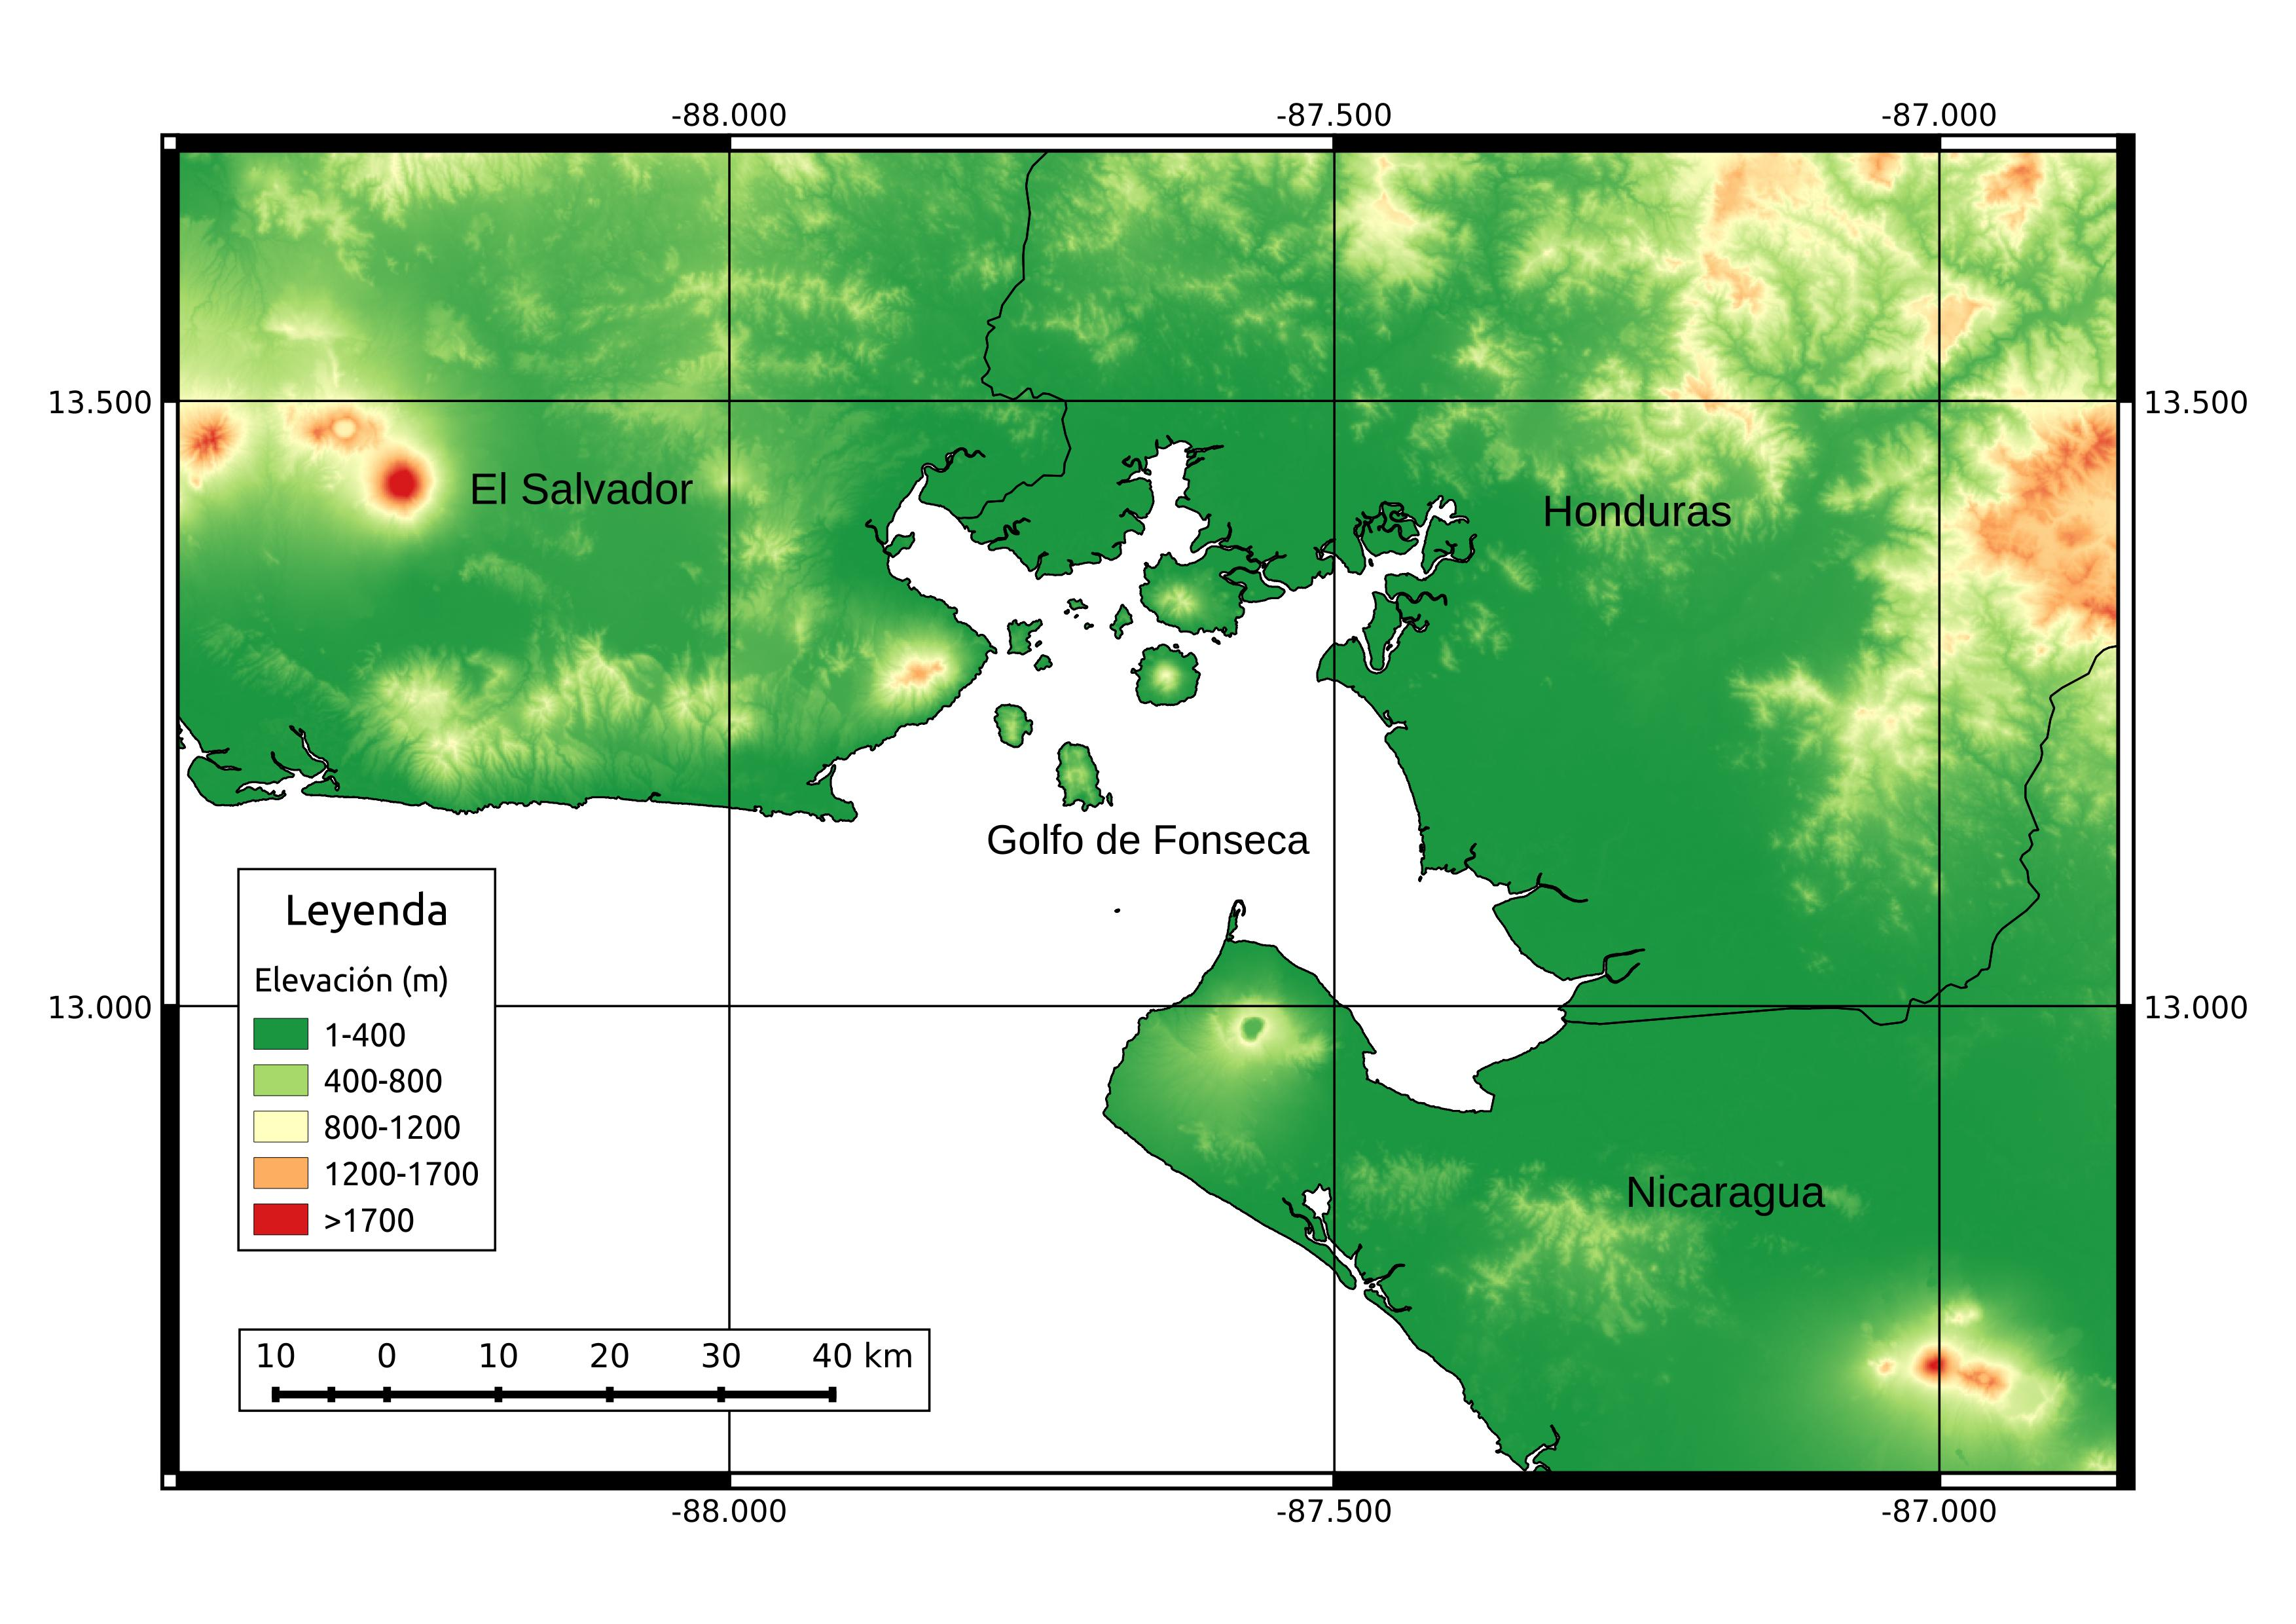
\includegraphics[width=0.8\linewidth]{./Imagenes/localizacion_elev.eps}
	\captionsetup{font={footnotesize,it}}
	\caption[Modelo de elevación del Golfo de Fonseca]{Modelo de elevación del Golfo de Fonseca. Fuente: Elaboración propia. Datos: \cite{SRTM2008}.}
	\label{fig:elevacion}
\end{figure}

De toda el área forestal de Honduras, que se sitúa en torno a las $54000000000 km^{2}$, los manglares ocupan alrededor de un 1.0\% $515781800 km^{2}$ \citep{anuario2013}. La mayor parte de este porcentaje de manglar se localiza en la costa pacífica del país, en el Golfo de Fonseca, que posee gran riqueza y diversidad de recursos naturales que están amenazados por su sobreexplotación \citep{Jimenez1994}. Esto hace que figure en la lista Ramsar de humedales protegidos a escala mundial \citep{Ramsar2014}. En total cuenta con 409 km de costa abarcando una extensión de $547 km^{2}$.\Sep

El Golfo de Fonseca, caracterizado por tener unas aguas poco profundas, que oscilan entre los 30m y 10m de máxima y 0.5m de mínima, está formado por una serie de ecosistemas interrelacionados formados por estuarios interiores, manglares, costas continentales e insulares. Las cuencas del Río Goascorán y el Río Negro son transfronterizas; la primera es compartida por El Salvador y Honduras y la segunda por Honduras y Nicaragua. Es pues un espacio internacional con humedales compartidos, lo que le otorga una importancia mayor a la hora de ser gestionado.\Sep

Cabe destacar que en 1998 el huracán Mitch devastó una extensa superficie del ecosistema del Golfo de Fonseca causando incontables pérdidas humanas y económicas y cubriendo de lodo las zonas de manglar llegando a provocar un ligero cambio en la línea de costa debido a las crecidas de los ríos y a las amplias mareas \citep{mexico1999honduras}.

\section{Bases teóricas de teledetección} \label{sec:bases}
\subsection{Fundamentos} \label{subsec:fundamentos}
La teledetección es la técnica que nos permite obtener información de los objetos situados en la superficie de la Tierra realizando una observación remota \citep{Curran1991Longman} \citep{chuvieco2002teledeteccion} \citep{schowengerdt2006}. Para que esta observación sea posible debe haber algún tipo de nexo entre el objeto y el sistema sensor u observador. De esta afirmación se extraen los tres elementos básicos de la teledetección: el objeto observado, el sensor y el el flujo energético que los relaciona.\Sep

Hay tres formas de que un sensor pueda adquirir la información del objeto. Estas son: por reflexión, por emisión y por emisión-reflexión.\Sep

\begin{figure}
	\centering
	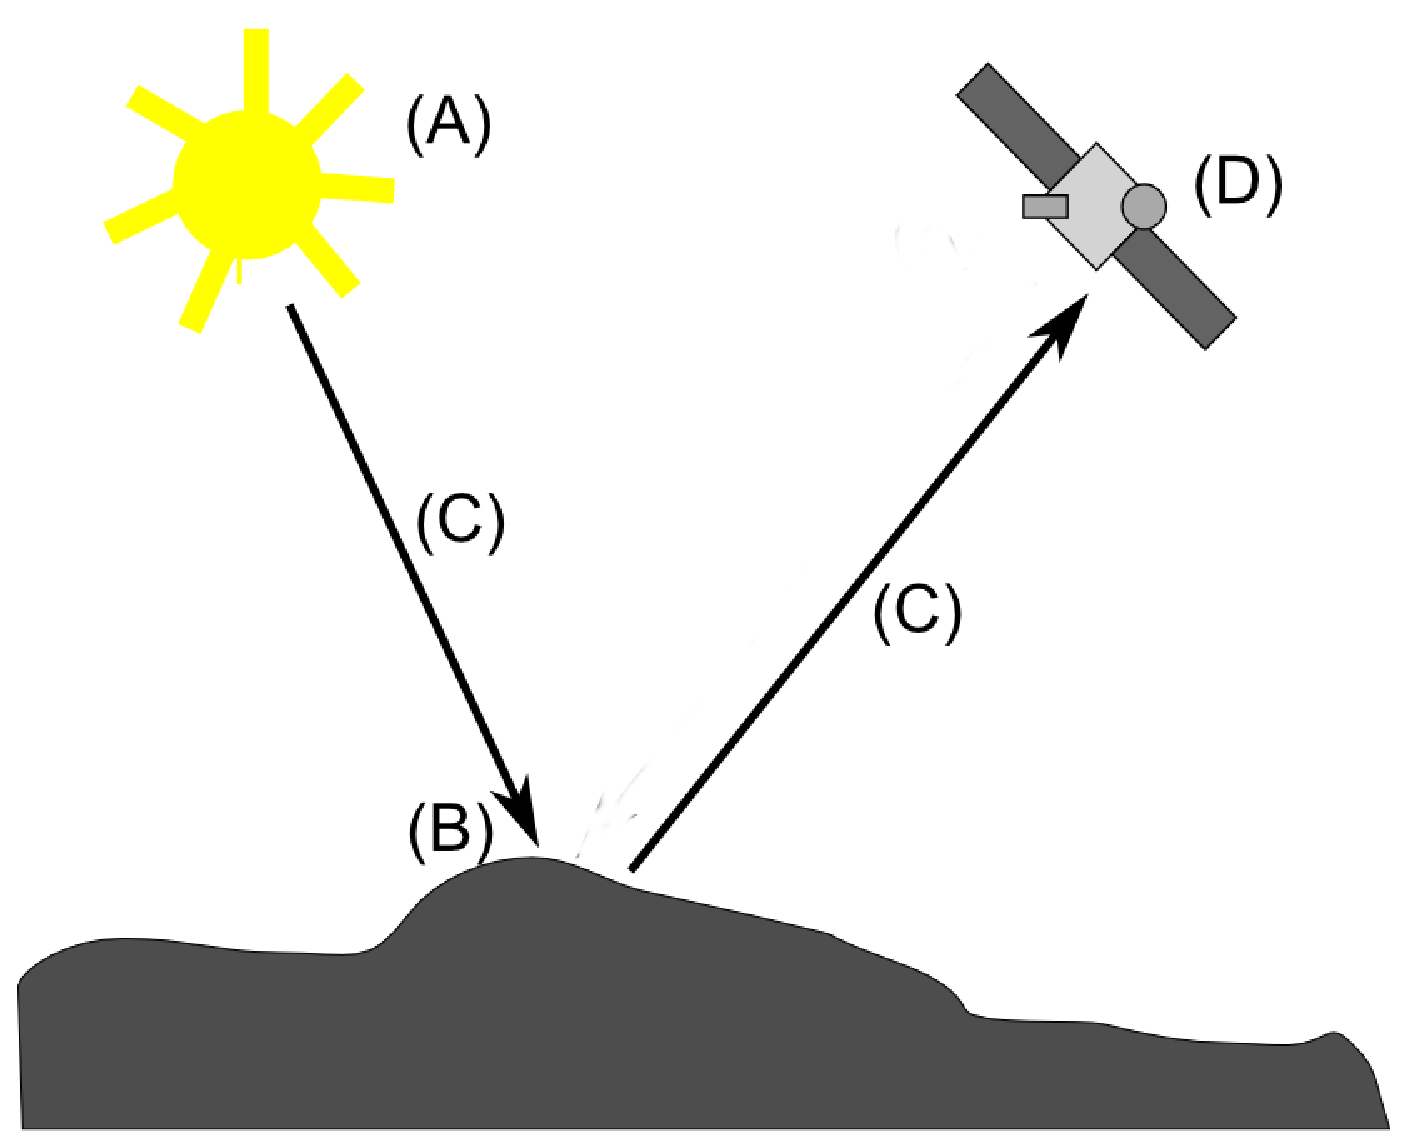
\includegraphics[width=0.4\linewidth]{./Imagenes/Elementos_teledeteccion_modificado.eps}
	\captionsetup{font={footnotesize,it}}
	\caption[Elementos de teledetección]{Elementos de teledetección. Fuente: \cite{Olaya2010}.}
	\label{fig:elementos}
\end{figure}

La primera forma deriva directamente de la reflexión solar (será la empleada en este \ac{TFG}) como se muestra en la figura \ref{fig:elementos}. El Sol (A) ilumina la superficie terrestre que refleja esa energía (C) en función del tipo de cubierta (B). El flujo reflejado es recogido por el sensor (D) que, de ser portado por un satélite, debe atravesar una capa de atmósfera que dispersa y absorbe parte de la señal. El flujo energético entre la cobertura y el sensor constituye una forma de radiación electro-magnética \citep{Olaya2010}.\Sep

\subsection{Espectro Electro-magnético}
Podemos definir cualquier tipo de energía en función de su longitud de onda, de la que se establecen una serie de bandas en donde la radiación electro-magnética manifiesta un comportamiento similar. Esta organización en bandas se denomina espectro electro-magnético (figura \ref{fig:espectro}). Esta comprende desde longitudes de onda corta, como los rayos gamma ($\gamma$) con menos de $10^{-11} m$, a longitudes de onda mayores de un metro como las ondas de radio.\Sep

\begin{figure}
	\centering	
	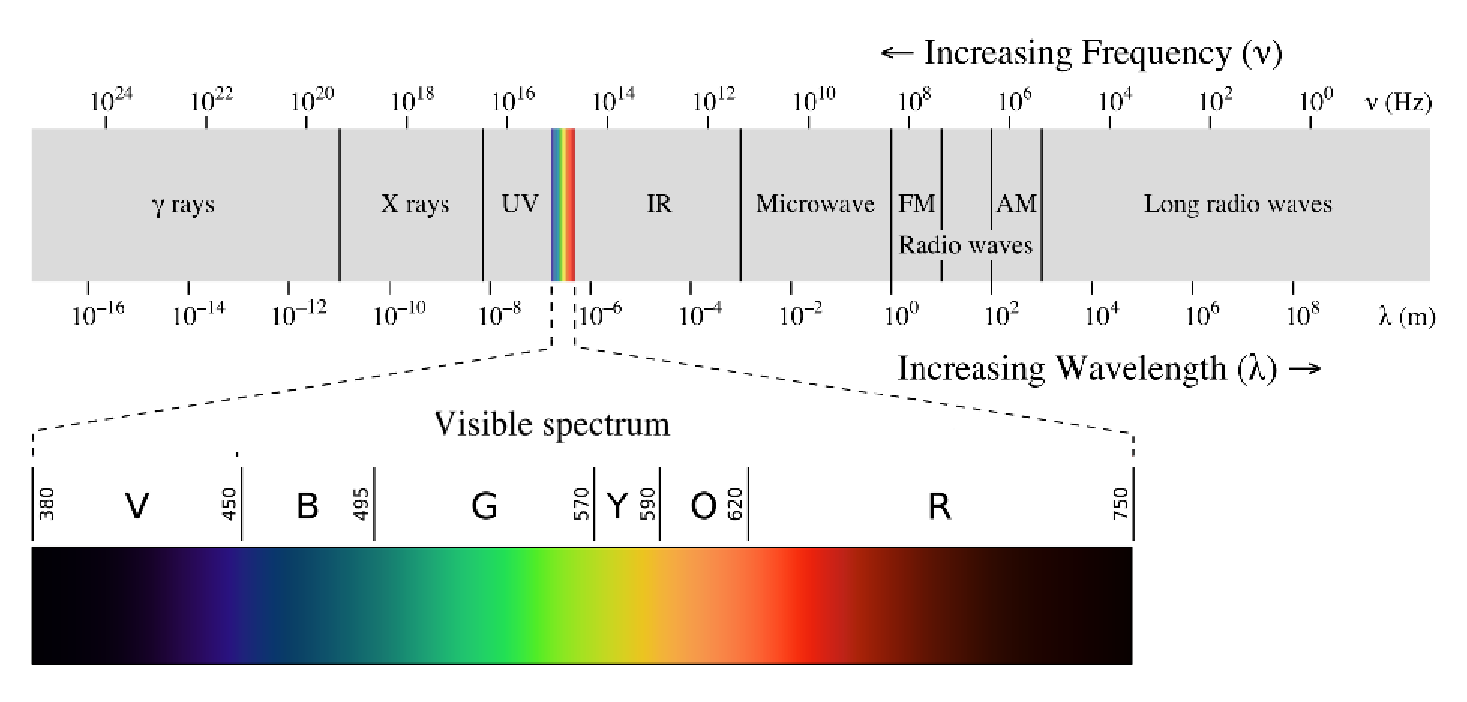
\includegraphics[width=0.9\linewidth]{./Imagenes/Espectro.eps}
	\captionsetup{font={footnotesize,it}}
	\caption[Espectro electro-magnético]{Espectro electro-magnético. Fuente: Wikimedia Commons.}
	\label{fig:espectro}
\end{figure}

En el cuadro \ref{tab:bandas} se destacan la serie bandas espectrales más empleadas en teledetección, siendo su denominación y ancho de banda el generalizado.\Sep

\begin{table}\centering
	\caption[Bandas espectrales utilizadas en teledetección]{Bandas espectrales utilizadas en teledetección.}
	\begin{tabular}{@{}llc@{}}
		\toprule[0.4mm]
		\multicolumn{2}{c}{\textbf{Banda}} & \textbf{L. de onda} \\
		\midrule
		\multirow{3}{*}{Visible} & Azul & $0.4-0.5{\mu}m$ \\
		& Verde & $0.5-0.6{\mu}m$ \\
		& Rojo & $0.6-0.7{\mu}m$ \\
		\midrule
		\multirow{3}{*}{Infrarrojo} & Cercano (IRC) & $0.7-1.2{\mu}m$ \\
		& Medio (IRM) & $1.2-8.0{\mu}m$ \\
		& Térmico (IRT) & $8.0-14.0{\mu}m$ \\
		\midrule
		\multicolumn{2}{c}{Microondas (M)} & $>1mm$\\
		\bottomrule[0.4mm]
	\end{tabular}
	\label{tab:bandas}
\end{table}

El espectro visible es la única radiación electromagnética perceptible por la vista. Como se muestra en el cuadro \ref{tab:bandas} esta banda se divide en otras tres elementales: azul, verde y rojo; en razón de los colores primarios que los ojos perciben a esas longitudes de onda.\Sep

En el caso de la banda infrarroja esta también se divide en tres bandas elementales: \ac{IRC}, \ac{IRM} e \ac{IRT}. El \ac{IRC}, también denominado próximo, es de especial importancia puesto que es utilizado para detectar masas vegetales y concentraciones de humedad. En el \ac{IRM} tenemos que diferenciar el \ac{SWIR} o infrarrojo de onda corta (situado entre 1.2 y 2.5$\mu$m resultando una banda indicada para estimar el contenido en humedad de la vegetación y los suelos) y el \ac{IRM} propiamente dicho (situado entre 2.5 y 8$\mu$m siendo determinante para la detección de focos de alta temperatura como incendios).\Sep

El \ac{IRT} es el indicado para dimensionar las emisiones de temperatura de las cubiertas sobre la superficie terrestre. Es poco utilizado para otros fines.\Sep

Las microondas tienen interés por ser un tipo de energía capaz de penetrar la cubierta nubosa pero no se tendrá en cuenta en este tipo de trabajos.\Sep

En capítulos sucesivos veremos que los valores de los intervalos de longitudes de onda de las bandas tomadas por los sensores satelitales son ligeramente diferentes a los mostrados en este capítulo.

\subsection{Términos y Unidades}
Como se indicó anteriormente, para que se pueda producir la observación remota es preciso que el sensor detecte un flujo energético proveniente de las cubiertas sobre la superficie terrestre. Este flujo energético tiene una intensidad determinada que proviene o está dirigida a una cubierta determinada con una dirección concreta. Se definen a continuación las magnitudes absolutas empleadas en teledetección.

\begin{itemize}
	\item Energía radiante (Q). Indica el total de energía radiada en todas las direcciones. Es medida en Julios (J).
	\item Flujo radiante ($\phi$). Es el total de energía radiada en todas las direcciones por unidad de tiempo. Es medida en vatios (W). Se compone de flujo reflejado ($\phi_{r}$), flujo absorbido ($\phi_{a}$) y flujo transmitido ($\phi_{t}$).
	\item Emitancia radiante (M). Es el total de energía radiada en todas las direcciones por superficie y por unidad de tiempo. Es medida en vatios por metro cuadrado ($Wm^{-2}$).
	\item Irradiancia (E). Es el total de energía radiada sobre una unidad de superficie y por unidad de tiempo. Es equivalente a la emitancia, excepto a que se refiere a la energía incidente y no a la emitida. Es medida en $Wm^{-2}$.
	\item Intensidad radiante (I). Es el total de energía radiada por unidad de tiempo y por ángulo sólido ($\Omega$). Este ángulo es tridimensional y refiere a la sección completa de la energía transmitida (es medido en estéreo-radianes. La intensidad radiante se mide en vatios por estéreo-radian ($Wsr^{-1}$).
	\item Radiancia (L). Es el total de energía radiada en una determinada dirección por unidad de superficie y por ángulo sólido de medida. Es uno de los términos más importantes en teledetección porque es la magnitud que mide el sensor. Se cuantifica en vatio por metro cuadrado y estéreo-radián ($Wm^{-2}sr^{-1}$).
	\item Radiancia espectral ($L_{\lambda}$). Indica el total de energía radiada en una determinada longitud de onda por unidad de área y por ángulo sólido de medida.
\end{itemize}

De igual forma se definen magnitudes relativas que son adimensionales:

\begin{itemize}
	\item Emisividad ($\epsilon$). Es la relación entre la emitancia de la superficie (M) y la emitancia de un emisor perfecto (cuerpo negro) a igual temperatura.
	\item Reflectividad ($\rho$). Es la relación entre el flujo reflejado y el incidente.
	\item Absortividad ($\alpha$). Es la relación entre el flujo absorbido y el incidente.
	\item Transmisividad ($\tau$). Relación entre el flujo transmitido y el incidente.
\end{itemize}

Debido a que la radiancia que capta un sensor depende de la que refleja la cubierta en la que incide, para detectar una cubierta por teledetección se precisa explicar como interactúa con la radiación solar incidente. El flujo incidente ($\phi_{i}$), como ya se mencionó, se descompone en tres términos: flujo reflejado ($\phi_{r}$), flujo absorbido ($\phi_{a}$) y flujo transmitido ($\phi_{t}$), es decir:
\begin{equation}
	\phi_{i}=\phi_{r}+\phi_{a}+\phi_{t}
	\label{eq:flujoinc}
\end{equation}
que expresado en términos relativos:
\begin{equation}
	\frac{\phi_{i}}{\phi_{i}}=\frac{\phi_{r}}{\phi_{i}}+\frac{\phi_{a}}{\phi_{i}}+\frac{\phi_{t}}{\phi_{i}}
	\label{eq:flujorel}
\end{equation}
lo que es igual a la suma de la reflectividad, absortividad y transmisividad ha de ser igual a uno:
\begin{equation}
	1=\rho+\alpha+\tau
	\label{eq:flujo}
\end{equation}
que variando según la longitud de onda ($\lambda$) bastaría con expresarlo de la siguiente manera:
\begin{equation}
	1=\rho_{\lambda}+\alpha_{\lambda}+\tau_{\lambda}
	\label{eq:flujolong}
\end{equation}

La cantidad de flujo incidente que es reflejado, transmitido y absorbido dependen directamente de las características de la cubierta que se está observando y de la longitud de onda a la que se observa. Para conocer fielmente las características de una cubierta conviene observarla a distintas longitudes de onda, lo que permitirá diferenciarla de otras cubiertas susceptibles de ser espectralmente similares.\Sep

La variación de longitud de onda, por ejemplo en el espectro visible, se detecta fácilmente pues se ve afectado en nada menos que el color en el que observamos. Un objeto será rojo, verde o azul si refleja la energía de la banda del espectro correspondiente o si absorbe más intensamente la de las otras bandas.\Sep

El flujo de energía recibida por el sensor depende, además de la reflectividad de la cubierta, de las condiciones atmosféricas, el emplazamiento ambiental de la cubierta y la geometría de la observación. El sensor puede registrar distintos valores para el mismo tipo de cubierta dependiendo de la variación en las condiciones de observación o iluminación. Hay que tener en cuenta que una cubierta vegetal presenta distintos estados biológicos a lo largo del año, lo que añade una componente temporal a la toma de datos. En resumen, los factores que afectan a las características espectrales de una cubierta son:
\begin{itemize}
	\item Ángulos de iluminación y observación, que varían con la latitud, fecha del año y hora de la observación y la posición del sensor.
	\item Modificaciones que el relieve introduce en el ángulo de iluminación, como pueden ser la orientación de las laderas de una montaña o pendientes.
	\item Influencia de la atmósfera, absorción por nubes y dispersión selectiva en distintas longitudes de onda.
	\item Variaciones medioambientales en la cubierta: asociación con otras superficies, homogeneidad que presenta o estado fenológico entre otras.
	\item Sustrato edafológico o litológico, especialmente influyente cuando la cubierta observada presenta una densidad media.
\end{itemize}

\subsection{Firmas espectrales}
Las firmas o signaturas espectrales (figuras \ref{fig:firma} y \ref{fig:biblioteca_esp}), extraído del inglés \textit{spectral signatures}, es la forma de reflejarse que tiene una cubierta a lo largo de distintas longitudes de onda y se utiliza para discriminar una cubierta de otra a partir de una observación remota. Son fundamentales para reconocer cubiertas de interés o extraer parámetros o características intrínsecas a dicha cubierta. La firma espectral se puede obtener de las siguientes fuentes:

\begin{itemize}
	\item Medidas con un radiómetro.
	\item Bibliotecas espectrales.
	\item Simulaciones mediante modelos físicos.
	\item Imagen con la debida resolución espectral.
\end{itemize}

El medio más sencillo de disponer de firmas espectrales son las bibliotecas espectrales. Las bibliotecas espectrales son colecciones de firmas espectrales, tomadas en condiciones controladas por radiómetros en laboratorio, que sirven de referencia para conocer el comportamiento de una cubierta determinada \citep{andinofase1}.

\begin{figure}
	\centering	
	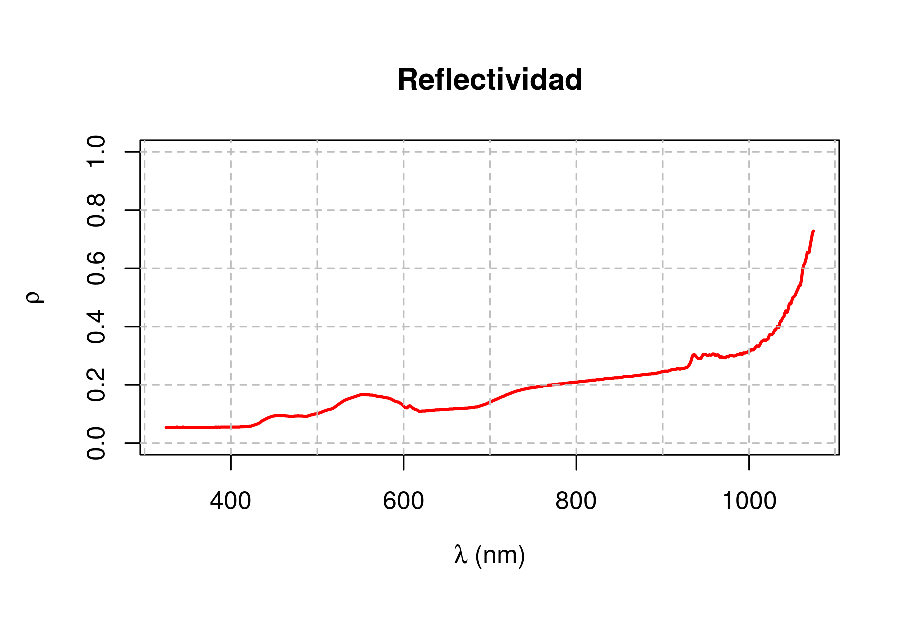
\includegraphics[width=0.7\linewidth]{./Imagenes/Firma_espectral.eps}
	\captionsetup{font={footnotesize,it}}
	\caption[Firma espectral ejemplo]{Firma espectral ejemplo de una cubierta no identificada. Fuente: Elaboración propia.}
	\label{fig:firma}
\end{figure}

Hay numerosos ejemplos de bibliotecas espectrales en Internet, como las del \ac{SIGFIRM} venezolano que recoge el comportamiento espectral de los cultivos en regiones agrícolas de Venezuela \ref{fig:biblioteca_esp}; o la ASTER spectral library de la NASA, que recoge datos de otras tres bibliotecas espectrales: las del \ac{JHU}, \ac{JPL} y \ac{USGS} registrando más de 2400 firmas de materiales como minerales, rocas, suelos y algunas cubiertas artificiales como lo son cemento, aluminio o papel.\Sep

\begin{figure}
	\centering
	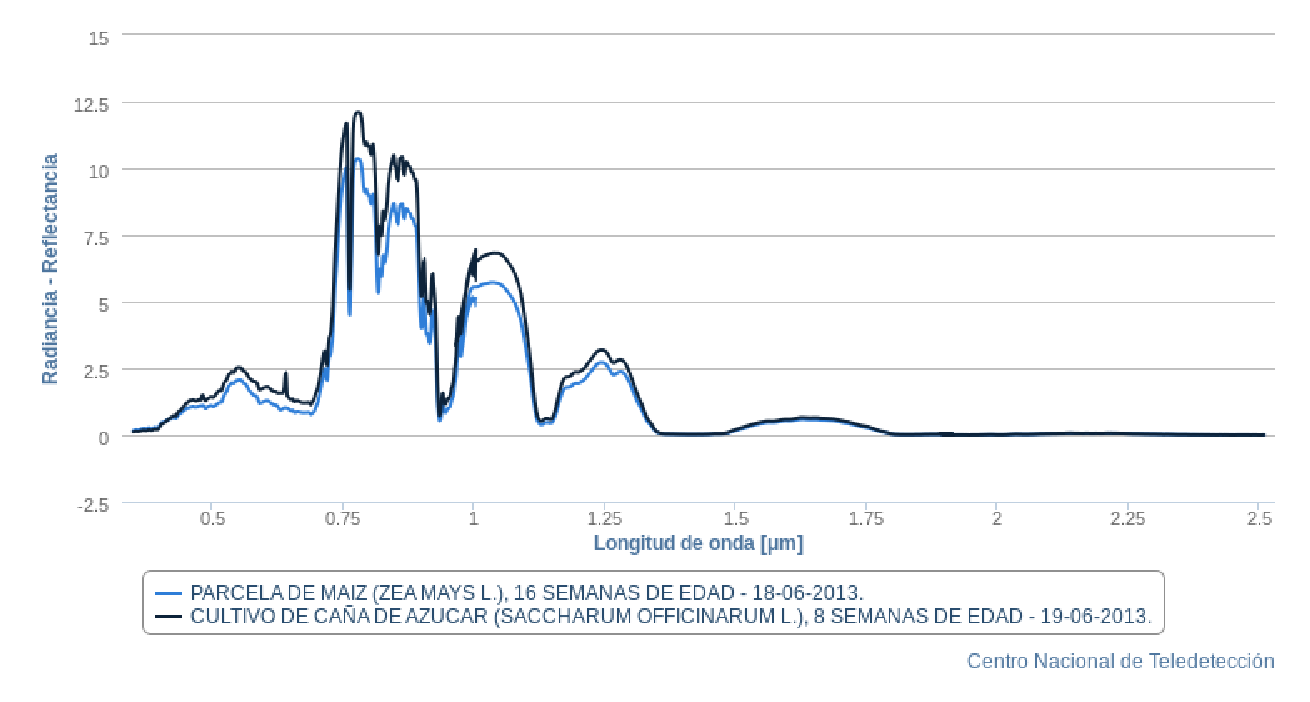
\includegraphics[width=0.7\linewidth]{./Imagenes/biblioteca_espectral_SIGFIRM.eps}
	\captionsetup{font={footnotesize,it}}
	\caption[Biblioteca espectral SIGFIRM]{Biblioteca espectral de maíz y caña de azucar. Fuente: \ac{SIGFIRM}}
	\label{fig:biblioteca_esp}
\end{figure}

\subsection{Sensores}
\label{subsec:sensores}
En el apartado de fundamentos (\ref{subsec:fundamentos}) de este mismo capítulo se indicaba que el sistema sensor era una de los tres componentes principales de la teledetección.\Sep

La clasificación más común de los sensores es según la forma de recibir la energía de las cubiertas, dando lugar a:
\begin{itemize}
	\item Pasivos, donde el sensor recibe la energía emitida por un agente exterior (e.g. el Sol).
	\item Activos, donde el sensor recibe un haz de energía emitido por él mismo (e.g. radares).
\end{itemize}

\subsubsection{Sensores pasivos} \label{subsubsec:sensorespasivos}
En una clasificación más detallada de los sensores pasivos estos se dividen en sensores fotográficos (cámaras analógicas), óptico-electrónicos (exploradores de barrido, de empuje y cámaras de vídeo) y de antena (radiómetros de microondas), en función del procedimiento que emplean para recibir la radiación procedente de los objetos.\Sep

Lo que concierne a este \ac{TFG} serán los sensores pasivos óptico-electrónicos ya que las cámaras analógicas eran más utilizadas en fotogrametría aérea y los radiómetros de microondas trabajan en frecuencias muy elevadas.\Sep

Los sensores óptico-electrónicos combinan una óptica similar a las cámaras analógicas con un sistema de detección electrónica permitiendo prescindir de un soporte sólido de grabación de imágenes. El sensor convierte la señal de radiancia proveniente del objeto en un valor digital. Los sensores exploradores de barrido, que son los más habituales, utilizan un espejo que oscila perpendicularmente a la dirección de la trayectoria.\Sep

Un ejemplo de sensor remoto pasivo de barrido es el \ac{ETM+} montado sobre el satélite Landsat 7. Otro ejemplo de explorador de barrido son los sensores \ac{TM} del Landsat 5, el \ac{OLI} del Landsat 8 (de cuyas imágenes se hará uso en este \ac{TFG} y se le dedicará un parágrafo) o el \ac{AVHRR} del NOAA. De los tres primeros se extraen los cuadros \ref{tab:sensoresTM}, \ref{tab:sensoresETM} y \ref{tab:sensoresOLI}.\Sep

\begin{table}
	\centering
	\caption[Bandas en el sensor TM]{Bandas en el sensor TM del proyecto Landsat. Fuente: USGS.}
	\begin{tabular}{@{}cccc@{}}
		\toprule[0.4mm]
		Banda & Nombre & L. onda ($\mu$m) & Resolución (m)\\
		\midrule
		1 & B & 0.45--0.52 & 30 \\
		2 & G & 0.52--0.60 & 30 \\
		3 & R & 0.63--0.69 & 30 \\
		4 & NIR & 0.76--0.90 & 30 \\
		5 & NIR & 1.55--1.75 & 30 \\
		6 & TIR & 10.40--12.50 & 120 \\
		7 & MIR & 2.08--2.35 & 30 \\
		\bottomrule[0.4mm]
	\end{tabular}
	\label{tab:sensoresTM}
\end{table}

\begin{table}
	\centering
	\caption[Bandas en el sensor ETM+]{Bandas en el sensor ETM+ del proyecto Landsat. Fuente: USGS.}
	\begin{tabular}{@{}cccc@{}}
		\toprule[0.4mm]
		Banda & Nombre & L. onda ($\mu$m) & Resolución (m)\\
		\midrule
		1 & B & 0.45--0.52 & 30 \\
		2 & G & 0.52--0.60 & 30 \\
		3 & R & 0.63--0.69 & 30 \\
		4 & NIR & 0.77--0.90 & 30 \\
		5 & NIR & 1.55--1.75 & 30 \\
		6 & TIR & 10.40--12.50 & 60 \\
		7 & MIR & 2.08--2.35 & 30 \\
		\bottomrule[0.4mm]
	\end{tabular}
	\label{tab:sensoresETM}
\end{table}

\begin{table}
	\centering
	\caption[Bandas en el sensor OLI]{Bandas en el sensor OLI del proyecto Landsat 8. Fuente: USGS.}
	\begin{tabular}{@{}cccc@{}}
		\toprule[0.4mm]
		Banda & Nombre & L. onda ($\mu$m) & Resolución (m)\\
		\midrule
		1 & Coastal & 0.43--0.45 & 30 \\
		2 & B & 0.45--0.51 & 30 \\
		3 & G & 0.53--0.59 & 30 \\
		4 & R & 0.64--0.67 & 30 \\
		5 & NIR & 0.85--0.88 & 30 \\
		6 & SWIR & 1.57--1.65 & 30 \\
		7 & SWIR & 2.11--2.29 & 30 \\
		9 & Cirrus & 1.36--1.38 & 30 \\
		\bottomrule[0.4mm]
	\end{tabular}
	\label{tab:sensoresOLI}
\end{table}

Otro tipo de sensor pasivo son los exploradores de empuje. En estos se elimina el espejo oscilante, en cuyo lugar se disponen una serie de detectores que cubren todo el campo de visión del sensor que exploran, en cada momento, una línea completa desplazándose esta línea simultáneamente con la plataforma. Estos exploradores permiten aumentar la resolución espacial y agilizan la detección de datos al hacer la conversión radiancia a valor digital por línea y no por píxel como los anteriores.\Sep

Ejemplos de exploradores de empuje son los sensores \ac{HRV} del SPOT o los senores portados por los satélites IKONOS o Quickbird.

\subsection{Resoluciones}

Se define la resolución del sistema sensor en teledetección como la capacidad para discriminar información de detalle en un objeto. Otra definición utilizada es la de valor mínimo determinado para alguna de las variables que definen a una imagen digital \citep{chuvieco2002teledeteccion} .\Sep

El concepto de información de detalle de la primera definición comprende tanto al detalle espacial que ofrece el sensor como a número y anchura de bandas espectrales, a su carencia temporal y a la capacidad para distinguir variaciones en la energía que detecta. Esto significa que el concepto de resolución se basa en el conjunto de:
\begin{enumerate}
	\item Resolución espacial.
	\item Resolución espectral.
	\item Resolución radiométrica.
	\item Resolución temporal.
\end{enumerate}

\subsubsection{Resolución espacial}
Designa el objeto más pequeño que es posible distinguir en la imagen digital. Se mide en milímetros sobre la imagen o metros sobre el terreno y depende de la longitud focal del sensor y altura sobre la superficie. En sensores óptico-electrónicos se utiliza el \ac{IFOV}, que se define como la sección angular que observa el sensor en un momento determinado.
\begin{equation}
	d=2h\tan(IFOV/2)
	\label{eq:res_esp}
\end{equation}
donde $d$ es la distancia sobre el terreno que abarca con ese ángulo \ac{IFOV}, y $h$ la altura del sensor sobre el terreno. Esta mínima unidad de información en la imagen es la que se denomina píxel.\Sep

La resolución espacial de un sensor, como ya se ha mencionado, depende de varios factores, como la altura orbital, la longitud focal y el número de detectores. En los sensores de antena, la resolución espacial depende del tamaño de la antena, la altura de la plataforma y el ángulo de incidencia.\Sep

Dependiendo de la resolución espacial tenemos cuatro tipos de sensores:
\begin{enumerate}
	\item De alta resolución. Con resoluciones próximas al metro de ancho.
	\item De recursos naturales. Con resoluciones entre los 25 x 25m y 1000 x 1000m.
	\item De baja resolución. Por lo general montados sobre satélites geoestacionarios y dedicados a ámbitos metorológicos, cuentan con una resolución espacial que puede llegar a los 5 x 5km.
\end{enumerate}

\subsubsection{Resolución espectral}
Designa el número y anchura de bandas espectrales que puede discriminar el sensor. Es muy importante la capacidad del sensor para registrar simultaneamente el comportamiento de un mismo objeto en varias bandas del espectro. En definitiva, un sensor tendrá mayor resolución cuanto mayor número de bandas detecte, facilitando así la caracterización espectral de las cubiertas.\Sep

Es evidente la importancia que tiene la elección del sensor en cuanto al número de bandas, ancho y longitud de las mismas dependiendo del objetivo del trabajo a realizar. Por ejemplo, para la detección de vegetación se hace más importante disponer de bandas del \ac{IRC} e \ac{IRM} más que del \ac{IRT}, en cambio para detectar incendios sí es importante disponer de la banda del \ac{IRT}.

\subsubsection{Resolución radiométrica}
Designa la sensibilidad del sensor o su capacidad para detectar las variaciones en la radiancia espectral. En los equipos digitales, como por ejemplo el sensor \ac{ETM+}, la imagen es codificada en un formato binario, por lo que la resolución radiométrica se identifica con el rango posible de valores que almacena el sensor, medido como el número de bits que necesita cada valor numérico para almacenarse. El mencionado \ac{ETM+} ofrece una resolución de 8 bits, es decir, 256 niveles por píxel.\Sep

La importancia de este tipo de resolución se hace patente a la hora de interpretar las imágenes, sobre todo cuando esta interpretación es digital, ya que el ordenador aprovecha todo el rango de resolución radiométrica.

\subsubsection{Resolución temporal}
Designa la frecuencia de cobertura que proporciona el sensor, es decir, la periodicidad con la que adquiere imágenes de la misma zona de la superficie terrestre. Esto depende de las características orbitales de la plataforma (altura, velocidad e inclinación) y del diseño del sensor (del ángulo total de apertura). La resolución temporal dependerá también de las condiciones atmosféricas puesto que una amplia cobertura nubosa impedirá la observación y dilatará dicha temporalidad.\Sep

Las variaciones en la resolución temporal responden al objetivo para el que esté diseñado el sensor, pudiendo llegar a los 15 o 30 minutos de los satélites meteorológicos como Meteosat y hasta los 15 o 31 días de los satélites de recursos naturales como el Landsat o Spot.

\subsubsection{Resolución angular}
Designa la capacidad de un sensor de tomar instantáneas de una misma porción de terreno desde distintas órbitas. Esto se relaciona con la resolución temporal en que, tomando el supuesto de que en un momento dado la cobertura nubosa impide la observación, el sensor tome la imagen desde una órbita cercana en otro lapso de tiempo inclinándose para poder hacerla. Esta capacidad reduce el efecto de reflectividad bidireccional que presentan algunas cubiertas y los efectos de absorción y dispersión de la atmósfera.\Sep

En el cuadro \ref{tab:resoluciones} se comparan las diferentes resoluciones de los principales sensores para fines medioambientales que hay actualmente en órbita.

\begin{table}[ht]
	\centering
	\caption[Resoluciones de varios sensores]{Resoluciones de varios sensores.}
	\begin{tabular}{@{}ccccc@{}}
	\toprule[0.4mm]
	& Landsat 8 & QuickBird & Spot 6 & IKONOS \\
	& OLI & & HRV & \\
	\midrule
	R. Espacial MS (m) & 30--60 & 2.44--2.88 & 6 & 3.2--4 \\
	R. Espectral (nm) & 450--12500 & 450--900 & 455--890 & 445--853 \\
	R. Radiométrica (bits) & 8 & 11 & 12 & 11 \\
	R. Temporal (días) & 16 & 1--3 & 1--3 & 3 \\
	\bottomrule[0.4mm]
	\end{tabular}
	\label{tab:resoluciones}
\end{table}

\subsection{Correcciones}
Como se exponía anteriormente la imagen digital tomada por el sistema sensor se compone de una malla de píxeles que toman un valor numérico concreto obtenido a partir de la radiancia observada. Ese valor numérico que codifica cada píxel es el llamado \ac{ND}. La propiedad más ventajosa de esos \ac{ND} es que pueden traducirse a color o niveles de gris, por ejemplo mediante el uso de un monitor, dependiendo, la intensidad, del \ac{ND}. A partir del \ac{ND} visualizado se pueden hacer operaciones de realce que no modificarán su valor pero sí harán que se vea con diferente intensidad. A este nuevo valor se le llamará \ac{NV}. El \ac{ND}, en cambio, es utilizado para operaciones de interpretación digital, especialmente cuando estas se relacionan con parámetros como la reflectividad o la temperatura.\Sep

La mejor forma de ver una imagen es como si fuera un sistema de tres dimensiones, donde las dos primeras dimensiones corresponden a la posición geográfica de la imagen y la tercera corresponde al \ac{ND}.\Sep

Las correcciones propiamente dichas son aquellos procesos con los que se eliminan anomalías detectadas en la imagen, tanto de localización como en la radiometría de los píxeles. La finalidad de estos procesos es la de disponer los datos de la forma más cercana a lo que sería una adquisición idónea (e.g. posición geográfica correcta). Es posible que la corrección más importante sea la geográfica, pues aporta validez cartográfica a los resultados y permite la conexión con otros datos geográficos en un \ac{SIG}.\Sep

Las principales fuentes de error que provocan la necesidad de realizar correcciones son:
\begin{itemize}
	\item Distorsiones originadas por la plataforma. El alabeo, el cabeceo o el giro lateral son movimientos que modifican la altitud de órbita del satélite, la velocidad o la orientación, lo que se traduce en problemas en la adquisición de las imágenes. Problemas como lo son cambios en la escala de adquisición o distorsiones en la geometría.
	\item Distorsiones provocadas por la rotación terrestre. En algunos sensores la toma de la imagen supera los 20 segundos, tiempo en el que la Tierra se desplaza en rotación unos 6 kilómetros.
	\item Distorsiones provocadas por el sensor. Distorsiones debidas al tipo de sensor relacionadas con el ángulo de barrido o el campo de visión global, provocando distorsiones cuanto más alejados están los píxeles del nadir.
	\item Distorsiones provocadas por la atmósfera. Los elementos de la atmósfera causan una modificación en la obtención de la señal original de la superficie terrestre. El efecto más importante es la dispersión, que implica un aumento de la señal recibida por el sensor.
\end{itemize}

La última de la distorsiones, la atmosférica, resulta importante de corregir para generar índices espectrales.\Sep

\subsubsection{Correcciones radiométricas}
Las correcciones radiométricas son aquellas técnicas que modifican los \ac{ND} originales con el objetivo de acercar su valor al que sería obtenido bajo condiciones ideales. Son correcciones radiométricas:
\begin{itemize}
	\item Restauración de líneas o píxeles perdidos. La imagen presenta líneas blancas o negras píxeles de aspecto contrastado al resto. Es una corrección aproximada, puesto que no se pueden poner píxeles de valor correcto donde no hay información.
	\item Corrección del bandeado de la imagen. Es especialmente perceptible en zonas de agua y problemático en los exploradores de empuje. Es un defecto periódico.
	\item Cálculo de reflectividades. Es una corrección muy importante para el análisis e interpretación de imágenes, pues como se decía anteriormente, es preferible trabajar con términos físicos que con \ac{ND}. Particularmente es importante a la hora de comparar datos con otros obtenidos con radiómetros de campo (uno de los objetivos de este \ac{TFG}).
	\item Cálculo de temperaturas.
	\item Detección de nubes.
\end{itemize}

\subsubsection{Correcciones geométricas}
Este tipo de correcciones incluyen los cambios en la posición que los píxeles ocupan en la imagen digital. Son correciones basadas en funciones numéricas que se aplican sobre la geometría de la imagen y la modifican.\Sep

\begin{eqnarray}
	f(c') & = & f_{1}(c,l) ; f(x,y) \\
	f(l') & = & f_{2}(c,l) ; f(x,y)
	\label{eq:correcgeom}
\end{eqnarray}\Sep

Las coordenadas columna y línea $c'$ y $l'$ de la imagen corregida son función de las coordenadas columna y línea de la imagen de entrada $c$ y $l$ o de las coordenadas del mapa al que se pretende superponer la imagen $x$ e $y$. Se trata de encontrar una relación que convierta los \ac{ND} de la imagen a su posición cartográfica en la proyección requerida (en este caso a la \ac{UTM}). Esto permite, entre otras cosas, hacer un mosaico con más imágenes para ampliar la cobertura de la imagen.\Sep

Hay dos procedimientos de corrección geométrica que se pueden aplicar a una imagen que se enumeran a continuación:

\begin{enumerate}
	\item Corrección a partir de modelos orbitales. Corrige los errores provocados por fuentes conocidas a partir de aplicar transformaciones inversas a las que realiza el sensor en el momento de la adquisición de los datos. Se necesita conocer con precisión las características orbitales de la plataforma y las especificaciones del sensor. Se corrigen de esta forma los errores sistemáticos
	\item Corrección a partir de puntos de control. Modela el error geométrico a partir de puntos de control repartidos a lo largo de la zona de la imagen. Estos puntos son de coordenadas conocidas y se asume que sean lo suficientemente representativos de las deformaciones de la imagen.
\end{enumerate}

El primero de los procedimientos es especialmente indicado para aquellas imágenes en las que no se pueden reconocer puntos de control, como imágenes marinas o con una amplia cobertura nubosa o bien sean imágenes con una resolución espacial en la que no se puedan establecer puntos de control con garantías. Por esta última razón es el tipo de corrección geométrica indicada para sensores de muy baja resolución espacial como los de plataforma de órbita geoestacionaria.\Sep

El método de corrección a partir de puntos de control requiere de la intervención humana, lo que resulta tedioso en comparación con el primer método. En cambio ofrece mayor precisión en la corrección dependiendo, evidentemente, de la medida en que en la imagen se puedan detectar los puntos de control establecidos.\Sep

\subsection{Clasificación de imágenes}
La clasificación es el último paso en el análisis de imágenes digitales mediante teledetección (se beneficia de los procesos de correcciones, realces y fusiones de imágenes) y de ella derivan los productos cartográficos finales en forma de mapas temáticos. El \ac{ND} pasa de reflejar el nivel de reflectancia a tener un valor categórico concreto que puede etiquetarse con un tipo concreto de superficie. Se genera así cartografía temática y facilita el trato estadístico de la información.\Sep

Hay numerosos métodos de clasificación que se desgranarán más adelante y que deben cumplir los siguientes requisitos:

\begin{itemize}
	\item Fiabilidad.
	\item Reproducible por otros con las mismas variables de entrada.
	\item Robustez. No debe ser sensible a pequeños cambios en las condiciones de entrada.
	\item Exhaustividad.
	\item Objetividad. No debe estar marcado por las decisiones del intérprete.
\end{itemize}

Uno de los problemas más comunes en la clasificación es la posible similitud entre dos o más cubiertas o inmersión de una sobre otra, que provoca que estas no se definan correctamente. Esto se podría solucionar ampliando la resolución espacial o aplicando la variable temporal a las imágenes (muy apto para discriminar masas vegetales debido a la evolución estacional). También se podría acudir a información auxiliar como topografía del terreno o tipos de suelo.

\subsubsection{Fases de la clasificación}
La clasificación consta de los siguientes puntos que dependiendo del tipo de clasificación, supervisada o no supervisada, se utilizarán de un modo u otro estas fases.
\begin{enumerate}
	\item Fase de entrenamiento.
Para la interpretación de la imagen es necesaria una experiencia previa que permita identificar las categorías según su textura, tono, tamaño o situación de los píxeles que la componen.

La finalidad de la fase de entrenamiento es definir un rango de valores de \ac{ND} que en conjunto describan las características de una cubierta concreta. A esto se le llama área de entrenamiento. Una cubierta no se define únicamente por un valor de \ac{ND} debido a la dispersión en el comportamiento espectral.

Se deberá seleccionar una muestra de píxeles de la imagen que representen lo más fielmente posible a la categoría de interés. A partir de esta muestra se podrán calcular los \ac{ND} medios y la variabilidad de cada categoría de las bandas que intervienen en la clasificación. Por lo tanto, las áreas de entrenamiento deben estar bien identificadas, deben ser suficientemente homogéneas y deben cubrir todas las clases.

En el método supervisado, se seleccionan los píxeles representativos teniendo en cuenta la experiencia en campo o el conocimiento previo del comportamiento espectral de las cubiertas por parte del usuario. Mientras, el método de clasificación no supervisado se basa en la búsqueda autónoma de las muestras dentro de la imagen.

El problema más común en la definición de clases es que el tipo de clase informacional (constituyen la leyenda del trabajo e.g. tipos de suelo) no corresponda con el tipo de clase espectral (ofrecen una respuesta espectral similar). Puede darse el caso de que una cubierta esté representada por varias clases espectrales, que varias cubiertas estén representadas por una sola clase espectral o que varias clases informacionales se correspondan con varias clases espectrales \citep{chuvieco2002teledeteccion}.

	\item Fase de asignación.
En esta fase a cada uno de los píxeles de la imagen se le asigna una clase obteniendo así una nueva imagen con los \ac{ND} expresando una categoría temática diferente. Los criterios de asignación definen un área de dominio, en torno al centro de cada categoría. Por lo tanto, si el \ac{ND} del píxel se encuentra dentro de esa área será asignado a esa clase.

Los clasificadores más habituales son:
\begin{itemize}
	\item Clasificador de mínima distancia: el píxel se asigna a la clase más cercana espectralmente.
	\item Clasificador de paralelepípedos: permite al usuario señalar los umbrales de dispersión espectral asociados a cada clase.
	\item Clasificador de máxima probabilidad (maximun likehood): el píxel se asigna a aquella clase con la que tenga mayor probabilidad de pertenencia.
\end{itemize}
	\item Obtención y presentación de resultados.
	\item Verificación de resultados.
\end{enumerate}